% Circumscribed Parallelepiped
% Author: Axel Pavillet
\documentclass[border=10pt]{standalone}
\usepackage{tkz-graph}
\usepackage{relsize}
\usetikzlibrary{arrows,decorations.markings,calc}

\definecolor{cd40000}{RGB}{212,0,0}
\definecolor{cffffff}{RGB}{255,255,255}
\definecolor{c2a7fff}{RGB}{42,127,255}
\definecolor{c0000d9}{RGB}{0,0,217}
\definecolor{c0000ff}{RGB}{0,0,255}

\usepackage{relsize}

% \tikzset{every path/.style={draw, ->,>=latex,line width=1pt,color=black}}

%\tikzset{every node/.style={draw,minimum width = 20pt,line width = 1.75pt,
%circle,inner sep=0pt,font = \fontsize{14}{14}\selectfont,fill=none}}
\newcommand{\n}{\text{\raisebox{0.3ex}{-}}}

\begin{document}

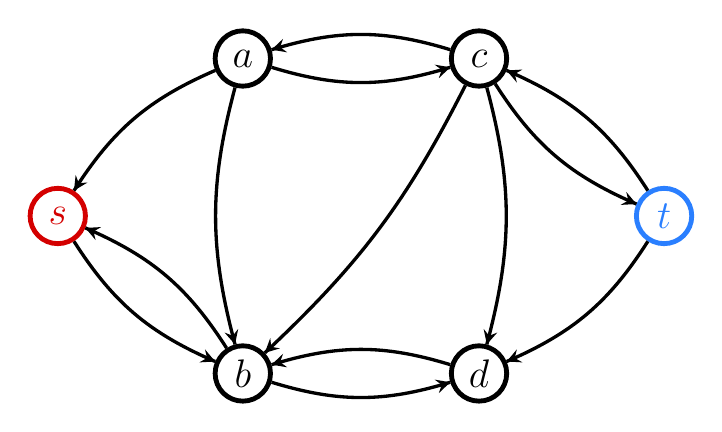
\begin{tikzpicture}[scale=0.5]

\begin{scope}[every node/.style={draw,minimum width = 20pt,line width = 1.75pt,
circle,inner sep=0pt,font = \fontsize{14}{14}\selectfont,fill=none}]
\node[color=cd40000] (s) at (-0.7,4) {$s$};
\node[color=c2a7fff] (t) at (14.7,4) {$t$};
%\node (e) at (7,4) {$e$};
\node (a) at (4,8) {$a$};
\node (c) at (10,8) {$c$};
\node (b) at (4,0) {$b$};
\node (d) at (10,0) {$d$};
\end{scope}

\begin{scope}[every node/.style={circle, fill=white, font=\fontsize{12}{12}\selectfont}]
% \node (sa) at (1.65,6) {$2/2$};
% \node (sb) at (1.65,2) {$7/9$};
% \node (ab) at (4,4) {$\n 3/3$};
% \node (ac) at (7,8) {$5/8$};
% \node (cb) at (7,4) {$\n 1/1$};
% \node (bd) at (7,0) {$3/9$};
% \node (dc) at (10,4) {$2/2$};
% \node (dt) at (12.35,2) {$1/1$};
% \node (ct) at (12.35,6) {$8/9$};

\node (sa) at (1.65,6) {};
\node (sb) at (1.65,2) {};
\node (ab) at (4,4) {};
\node (ac) at (7,8) {};
\node (cb) at (7,4) {};
\node (bd) at (7,0) {};
\node (dc) at (10,4) {};
\node (dt) at (12.35,2) {};
\node (ct) at (12.35,6) {};
\end{scope}

% \draw[->] (b) to [bend left=20.4]  node[midway, fill=white, font=\fontsize{12}{12}\selectfont] {$0/9$} (s);
% \draw[->] (s) to [bend left=20.4]  node[midway, fill=white, font=\fontsize{12}{12}\selectfont] {$3/9$} (b);
% \draw[->] (s) to [bend left=20]  node[midway, fill=white, font=\fontsize{12}{12}\selectfont] {$0/2$} (a);
% \draw[->] (a) to [bend left=20]  node[midway, fill=white, font=\fontsize{12}{12}\selectfont] {$0/2$} (s);
% \draw[->] (a) to [bend left=20]  node[midway, fill=white, font=\fontsize{12}{12}\selectfont] {$0/3$} (b);
% \draw[->] (b) to [bend left=18]  node[midway, fill=white, font=\fontsize{12}{12}\selectfont] {$3/3$} (a);
% \draw[->] (a) to [bend left=18]  node[midway, fill=white, font=\fontsize{12}{12}\selectfont] {$3/8$} (c);
% \draw[->] (c) to [bend left=20]  node[midway, fill=white, font=\fontsize{12}{12}\selectfont] {$0/8$} (a);
% \draw[->] (b) to [bend left=13]  node[midway, fill=white, font=\fontsize{12}{12}\selectfont] {$0/1$} (c);
% \draw[->] (c) to [bend left=13]  node[midway, fill=white, font=\fontsize{12}{12}\selectfont] {$0/1$} (b);
% \draw[->] (b) to [bend left=13]  node[midway, fill=white, font=\fontsize{12}{12}\selectfont] {$0/9$} (d);
% \draw[->] (d) to [bend left=20]  node[midway, fill=white, font=\fontsize{12}{12}\selectfont] {$0/9$} (b);
% \draw[->] (d) to [bend left=20]  node[midway, fill=white, font=\fontsize{12}{12}\selectfont] {$0/1$} (t);
% \draw[->] (t) to [bend left=13]  node[midway, fill=white, font=\fontsize{12}{12}\selectfont] {$0/1$} (d);
% \draw[->] (d) to [bend left=17]  node[midway, fill=white, font=\fontsize{12}{12}\selectfont] {$0/2$} (c);
% \draw[->] (c) to [bend left=17]  node[midway, fill=white, font=\fontsize{12}{12}\selectfont] {$0/2$} (d);
% \draw[->] (t) to [bend left=20]  node[midway, fill=white, font=\fontsize{12}{12}\selectfont] {$0/9$} (c);
% \draw[->] (c) to [bend left=20]  node[midway, fill=white, font=\fontsize{12}{12}\selectfont] {$3/9$} (t);

\usetikzlibrary{decorations.markings}

% \begin{scope}[very thick,decoration={
%     markings,
%     mark=at position 0.0 with {\arrow{stealth}}}
%     ]
%     % \draw[postaction={decorate}] (-4,0)--(4,0);
%     % \draw[postaction={decorate}] (4,0)--(4,2);
%     % \draw[postaction={decorate}] (4,2)--(-4,2);
%     % \draw[postaction={decorate}] (-4,2)--(-4,0);
%     \draw[postaction={decorate}] (sb) to (b);
%     \draw[postaction={decorate}] (sa) to (a);
%     % \draw[postaction={decorate}] (ab) to (b);
%     \draw[postaction={decorate}] (ac) to (c);
%     \draw[postaction={decorate}] (cb) to (b);
%     \draw[postaction={decorate}] (bd) to (d);
%     \draw[postaction={decorate}] (dc) to (c);
%     \draw[postaction={decorate}] (dt) to (t);
%     \draw[postaction={decorate}] (ct) to (t);
% \end{scope}


% \begin{scope}[very thick]
%   \draw (s) to (sb);
%   \draw (s) to (sa);
%   % \draw (a) to (ab);
%   \draw (a) to (ac);
%   \draw (c) to (cb);
%   \draw (b) to (bd);
%   \draw (d) to (dc);
%   \draw (c) to (ct);
%   \draw (d) to (dt);
% \end{scope}

%
% \draw[->] (s) to node[midway, fill=white, font=\fontsize{12}{12}\selectfont] {$3/9$} (b);
% \draw[->] (s) to node[midway, fill=white, font=\fontsize{12}{12}\selectfont] {$0/2$} (a);
% \draw[->] (a) to node[midway, fill=white, font=\fontsize{12}{12}\selectfont] {$0/3$} (b);
% \draw[->] (a) to node[midway, fill=white, font=\fontsize{12}{12}\selectfont] {$3/8$} (c);
% \draw[->] (b) to node[midway, fill=white, font=\fontsize{12}{12}\selectfont] {$0/1$} (c);
% \draw[->] (b) to node[midway, fill=white, font=\fontsize{12}{12}\selectfont] {$0/9$} (d);
% \draw[->] (d) to node[midway, fill=white, font=\fontsize{12}{12}\selectfont] {$0/1$} (t);
% \draw[->] (d) to node[midway, fill=white, font=\fontsize{12}{12}\selectfont] {$0/2$} (c);
% \draw[->] (c) to node[midway, fill=white, font=\fontsize{12}{12}\selectfont] {$3/9$} (t);
%
% \draw [gray,transform canvas={xshift=-0.3em,yshift=-0.3em},dash pattern=on 3pt off 2pt,postaction={decorate,decoration={markings,mark=between positions 3pt and 1 step 5pt with {\arrow{>};}}}] (s) to (sb);
%
% \draw [gray,transform canvas={xshift=-0.3em,yshift=-0.3em},dash pattern=on 3pt off 2pt,postaction={decorate,decoration={markings,mark=between positions 3pt and 1 step 5pt with {\arrow{>};}}}] (sb) to (b);
%
% \draw [gray,transform canvas={xshift=0.5em},dash pattern=on 3pt off 2pt,postaction={decorate,decoration={markings,mark=between positions 3pt and 1 step 5pt with {\arrow{>};}}}] (b) to (ab);
%
% \draw [gray,transform canvas={xshift=0.5em},dash pattern=on 3pt off 2pt,postaction={decorate,decoration={markings,mark=between positions 3pt and 1 step 5pt with {\arrow{>};}}}] (ab) to (a);
%
% \draw [gray,transform canvas={yshift=0.5em},dash pattern=on 3pt off 2pt,postaction={decorate,decoration={markings,mark=between positions 3pt and 1 step 5pt with {\arrow{>};}}}] (a) to (ac);
%
% \draw [gray,transform canvas={yshift=0.5em},dash pattern=on 3pt off 2pt,postaction={decorate,decoration={markings,mark=between positions 3pt and 1 step 5pt with {\arrow{>};}}}] (ac) to (c);
%
% \draw [gray,transform canvas={xshift=0.3em,yshift=0.3em},dash pattern=on 3pt off 2pt,postaction={decorate,decoration={markings,mark=between positions 3pt and 1 step 5pt with {\arrow{>};}}}] (c) to (ct);
%
% \draw [gray,transform canvas={xshift=0.3em,yshift=0.3em},dash pattern=on 3pt off 2pt,postaction={decorate,decoration={markings,mark=between positions 3pt and 1 step 5pt with {\arrow{>};}}}] (ct) to (t);
\begin{scope}[very thick,decoration={
    markings,
    mark=at position 0.99999 with {\arrow{stealth}}}]
\draw[postaction={decorate}] (s) to [bend right=17] (b);
\draw[postaction={decorate}] (b) to [bend right=17] (s);
% \draw[postaction={decorate}] (d) to [bend left=25] (b);
\draw[postaction={decorate}] (t) to [bend right=17] (c);
\draw[postaction={decorate}] (a) to [bend right=17] (c);
\draw[postaction={decorate}] (c) to [bend right=17] (a);
% \draw[postaction={decorate}] (a) to [bend right=25] (s);
% \draw[postaction={decorate}] (t) to [bend left=25] (d);
% \draw[postaction={decorate}] (c) to [bend left=25] (d);
% \draw[postaction={decorate}] (c) to [bend left=25] (b);
\draw[postaction={decorate}] (a) to [bend right=15] (b);
\draw[postaction={decorate}] (b) to [bend right=17] (d);
\draw[postaction={decorate}] (d) to [bend right=17] (b);
\draw[postaction={decorate}] (t) to [bend left=17] (d);
\draw[postaction={decorate}] (c) to [bend left=15] (d);
\draw[postaction={decorate}] (c) to [bend left=10] (b);
\draw[postaction={decorate}] (a) to [bend right=17] (s);
\draw[postaction={decorate}] (c) to [bend right=17] (t);
\end{scope}

\end{tikzpicture}
\end{document}
